
The cell populations studied by \citet{Dendrou:2009dv}, were obtained using manual gating in the FlowJo software\footnote{\url{www.flowjo.com}}.
Though ideally I would like to replace the entire manual gating process by an automatic algorithm I decided initially to concentrate on the two last univariate gating steps
to facilitate comparison with manual gating.


\subsection{The Manual Gating Approach }

The manual gating follows the current state of knowledge immune cell lineages (Figure~\ref{figure:manual-gating-strategy}).
Lymphocytes can be distinguished from more granular and larger cell types based on forward and side scatter.
Within the lymphocytes, the subset expressing CD4 are known as T lymphocytes.
The CD4+ T lymphocyte subset can be further divided into regulatory and non-regulatory cells (Figure~\ref{figure:lymphocyte-subsets}).
Regulatory cells represent a low frequency subset which are higher in CD25 and lower in CD127.
More precisely, regulatory T cells are further defined by an internal marker on the FOXP3 transcription factor.
Non regulatory T cells represent the bigger proportion of T lymphocytes.
They express more CD127 and less CD25 than regulatory T cells.
The non regulatory T cells can be further divided into naive and memory subsets (Figure~\ref{figure:manual-gating-strategy}d).
Naive and memory are transitional cell populations because naive cells turn into memory cells upon activation.
Typically as a result of the activation process, the CD45RA is lost so that consequently naive cells are higher in CD45RA than memory cells.
A further secondary distinguishable property is that memory cells tend to be higher in CD25 expression than naive cells.
Because CD25 expression on the naive cells is low, we may also define a threshold above which naive cells are deemed positive on CD25.
In the \citet{Dendrou:2009dv} study, this threshold is defined in terms of an isotype control (a sample not stained for CD25)
adjusted depending on the MFI of the blank beads population on that day.

The last two gating steps of the manual gating (Figure~\ref{figure:manual-gating-strategy}d) are examples of univariate gating which I have attempted to replace by automatic gating.
\begin{itemize} [noitemsep,topsep=0pt,parsep=0pt,partopsep=0pt]
\item On CD25 to threshold naive cells into positive and negative subsets.
\item On CD45RA to identify naive and memory cells within a two population mixture.
\end{itemize}

\begin{figure}
%\begin{center}
\centering
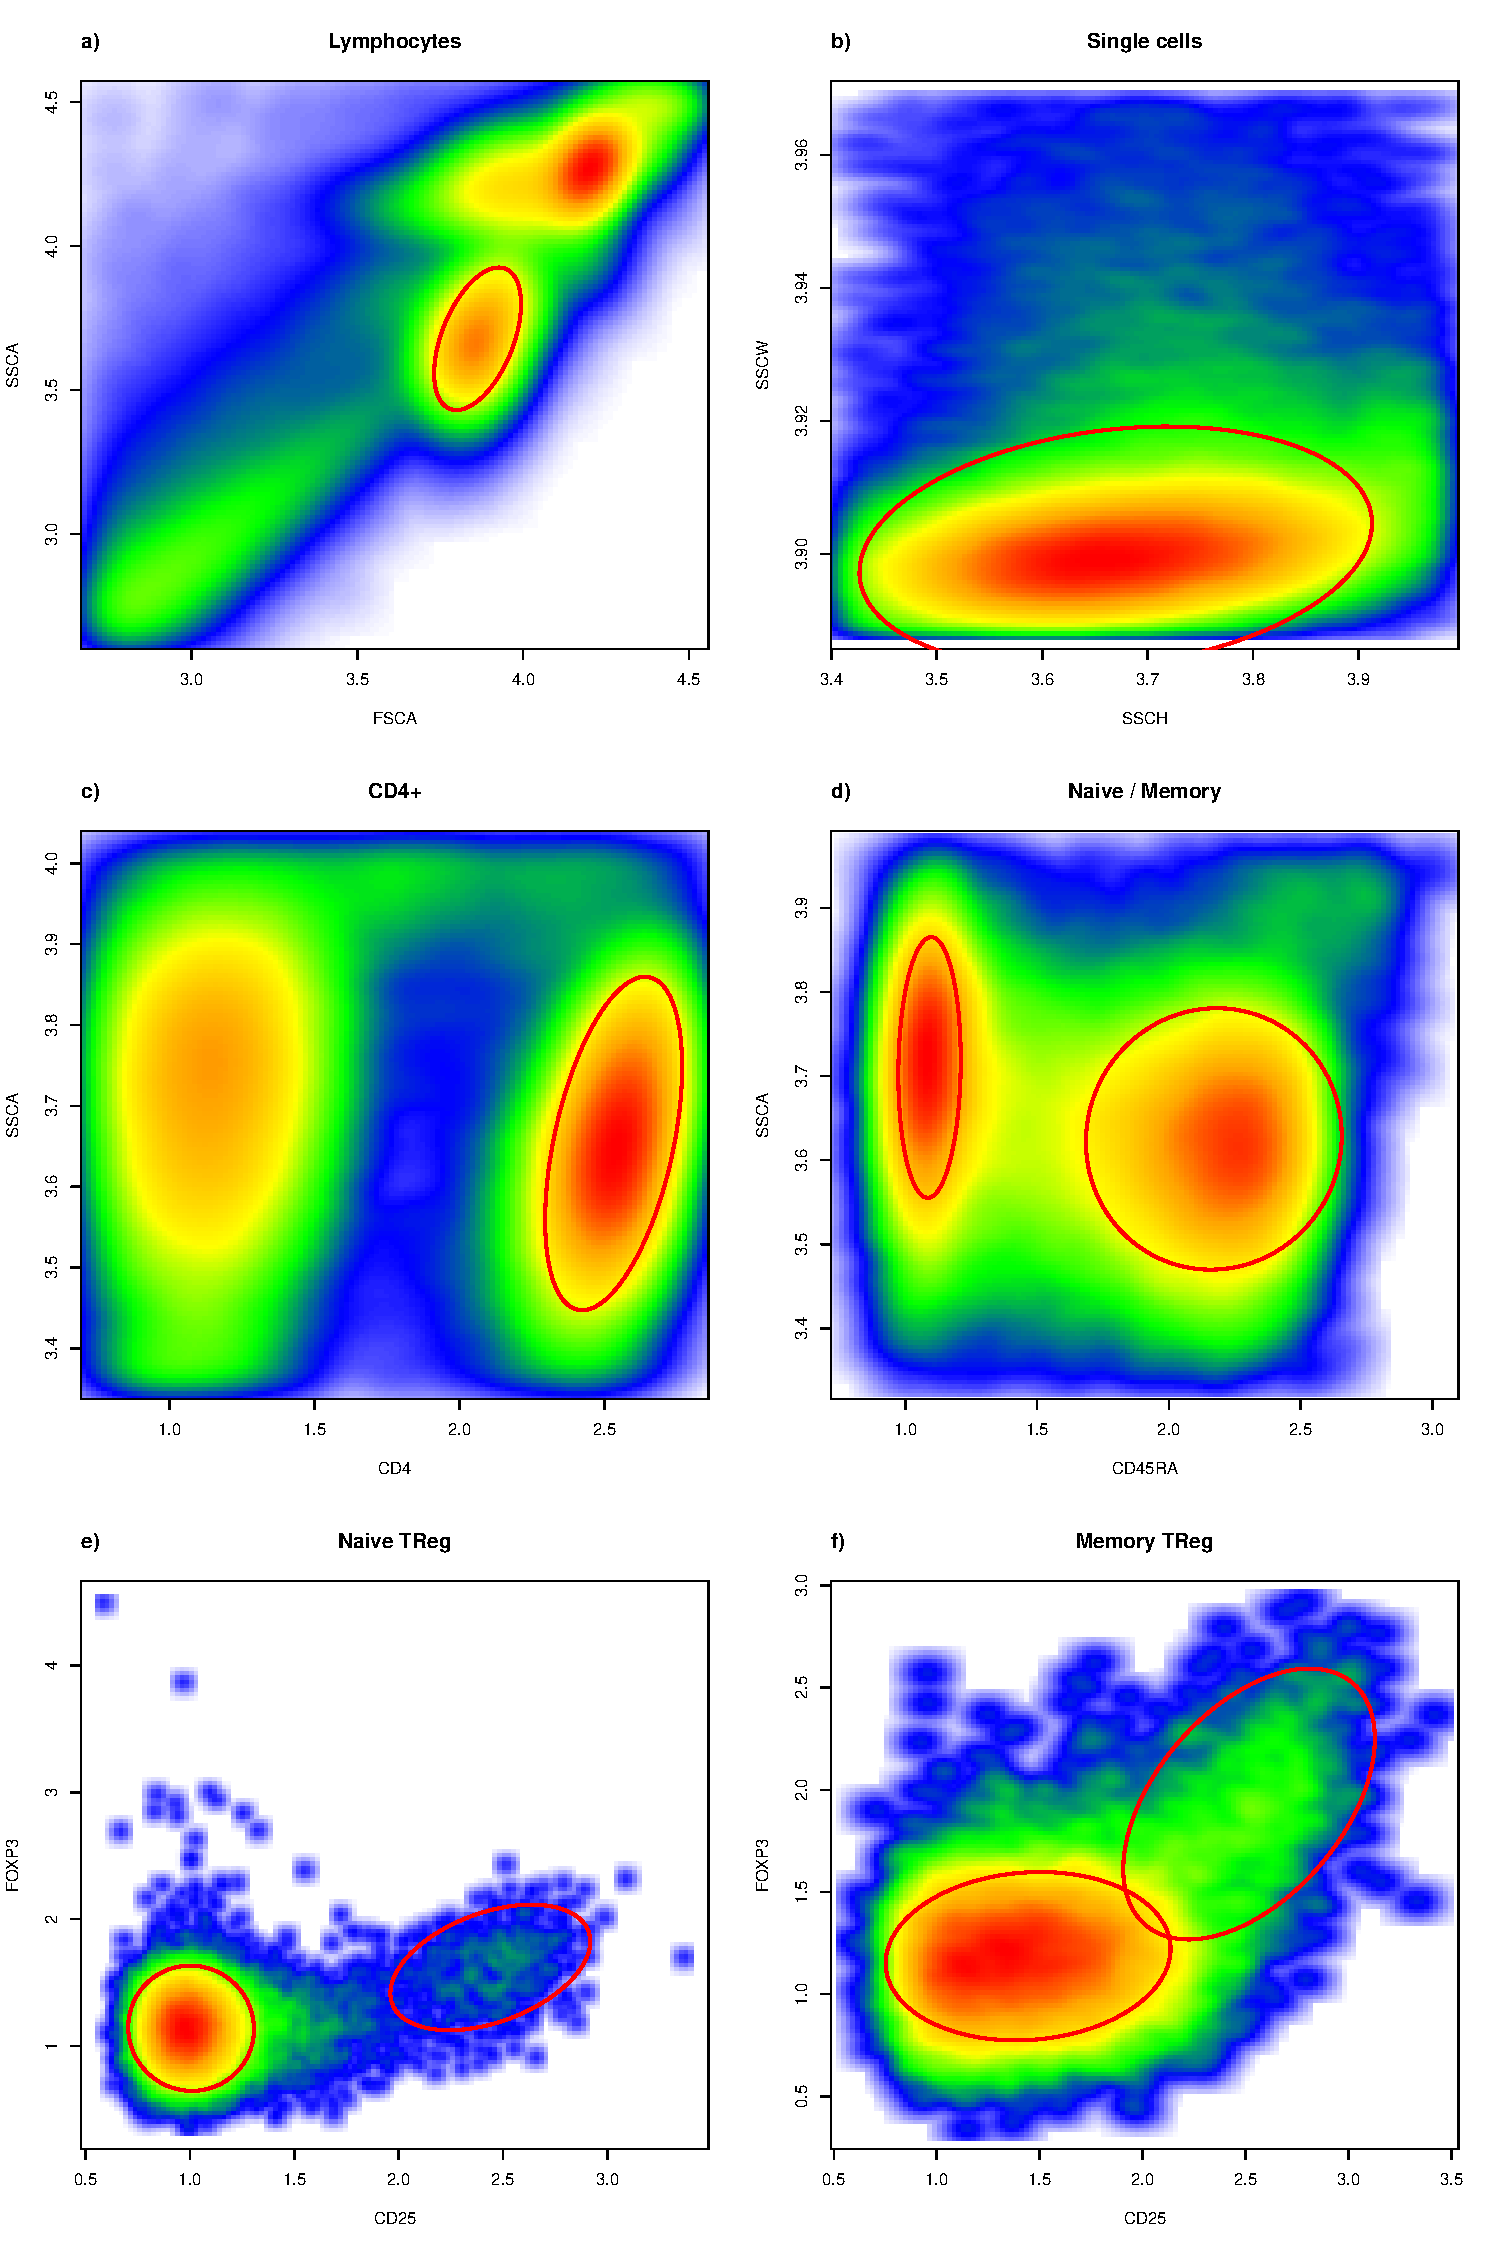
\includegraphics[scale=.5] {IL2RA/figures/ManualGating/manual-gating.pdf}
%\end{center}
\caption{Manual gating strategy to extract memory T cells and CD25+ naive T cells (green boxes). Note that the CD45RA gates exclude cells which are considered to be neither memory nor naive.
Our automated gating replaces the final stage of the manual gating on CD25 and CD45RA.}
\label{figure:manual-gating-strategy} 
\end{figure}

%%% Manual Gating Strategy
%\begin{figure} [ht]
%%\begin{center}
    %\begin{subfigure}[b]{.5\textwidth}
        %\includegraphics[scale=.5] {figures/ManualGating/manual1.pdf}
        %\caption{Lymphocyte Gate}
    %\end{subfigure}
    %~
    %\begin{subfigure}[b]{.5\textwidth}
        %\includegraphics[scale=.5] {figures/ManualGating/manual2.pdf}
        %\caption{CD4+ Gate}
    %\end{subfigure}
    %~
    %\begin{subfigure}[b]{.5\textwidth}
        %\includegraphics[scale=.5] {figures/ManualGating/manual3.pdf}
        %\caption{Non T Regs Gate}
    %\end{subfigure}
    %~
    %\begin{subfigure}[b]{.5\textwidth}
        %\includegraphics[scale=.5] {figures/ManualGating/manual4.pdf}
        %\caption{Naive/Memory Gate}
    %\end{subfigure}
%%\end{center}
%\caption{Manual gating strategy to extract memory T cells and CD25+ naive T cells.}
%\label{figure:manual-gating-strategy} 
%\end{figure}
%


\clearpage

\subsection{CD4 Lymphocyte Gating}

CD4 lymphocytes have well-known characteristics which makes them distinguishable based on their side, forward scatter and CD4 MFI.
This knowledge can be coded into our auto-gating in the form of a prior.

When the noise is excessive in a sample or the populations are rare, it is very difficult to identify accurately cell populations without sufficiently strong priors.

Lymphocytes typically represent $10\%$ of a whole blood sample but this can be much greater depending on how much debris is present in the sample.
For example if lysis was performed on the sample or if some hard cutoff was applied on the forward scatter at collection time,
then the sample would be enriched for lymphocytes as other cell types would be discarded.


The \Rpackage{flowClust} BioConductor R package \citet{Lo:2008it} allows to specify priors.
Priors define distributions over the parameters of the mixture models which can help speed up convergence of the EM algorithm.
Provided that overall the signal is sufficiently good in the majority of samples then an unbiased way of obtaining priors is to pool all samples together.
Realistically, each sample requires thinning before pooling, otherwise the resulting number of points would be too large for the EM algorithm.







